\documentclass[12pt]{beamer}

\usetheme{Oxygen}
\usepackage{thumbpdf}
\usepackage{wasysym}
\DeclareGraphicsRule{*}{mps}{*}{}
\usepackage{ucs}
\usepackage[utf8]{inputenc}
\usepackage{pgf,pgfarrows,pgfnodes,pgfautomata,pgfheaps,pgfshade}
\usepackage{verbatim}
\usepackage{pgfpages}
\usepackage{listings}
\usepackage{fix-cm}

\let\Tiny=\tiny

\lstset{
	language=C++,
	keywordstyle=\bfseries\ttfamily\color[rgb]{0,0,1},
	identifierstyle=\ttfamily,
	commentstyle=\color[rgb]{0.133,0.545,0.133}\itshape,
	stringstyle=\ttfamily\color[rgb]{0.627,0.126,0.941},
	showstringspaces=false,
	basicstyle=\small\ttfamily,
	numberstyle=\footnotesize,
	numbers=none,
	stepnumber=1,
	numbersep=10pt,
	tabsize=2,
	breaklines=true,
	prebreak = \raisebox{0ex}[0ex][0ex]{\ensuremath{\hookleftarrow}},
	breakatwhitespace=false,
	aboveskip={1.5\baselineskip},
	columns=fixed,
	%upquote=true,
	extendedchars=true,
	% frame=single,
	backgroundcolor=\color[rgb]{0.9,0.9,0.9},
	xleftmargin=2em,
	xrightmargin=2em,
}

\addtolength{\arraycolsep}{-3pt}

\definecolor{myblue}{rgb}{0.25, 0.25, 0.75}
\newcommand{\ct}[1]{\color{myblue} #1\color{black}}% Color text
\newcommand{\ctt}[1]{\color{red} #1\color{black}}% Color text
\newcommand{\myref}[1]{\ct{{\small[#1]}}}
\newcommand{\mycode}[1]{\texttt{\ctt{#1}}}

\newcommand{\be}{\begin{equation}}
\newcommand{\ee}{\end{equation}}
\newcommand{\om}{\omega}
\newcommand{\vp}{\varphi}
\newcommand{\ra}{\rightarrow}
\newcommand{\D}{\text{d}}
\newcommand{\I}{\text{i}}
\newcommand{\E}{\text{e}}
\newcommand{\paper}{paper\ }
\newcommand{\lpole}{\times}
\newcommand{\lsp}{*}
\newcommand{\mE}{\mathcal{E}}
\newcommand{\mU}{\mathcal{U}}
\newcommand{\reals}{\mathbb{R}}


\pdfinfo
{
  /Title       ( ``Loopy'' C/C++ programming)
  /Creator     (TeX)
  /Author      (Massimo Cavallaro)
}


\title[C++]{Programming seminar 2015 \\ Session 3: ``Loopy'' C/C++ }
%\subtitle{steady state and fluctuations}
\author{Massimo Cavallaro}
\institute[QMUL]{School of Mathematical Sciences\\
Queen Mary, University of London}
\date[4 March 2015]{4 March 2015}

\begin{document}
\defverbatim[colored]\LstIfElse{%
\begin{lstlisting}
if(cond1)
	{/* Runs iff cond1 true */}
else if(cond2)
	{/* Runs iff cond1 false and cond2 true */}
// Maybe more else-ifs, and maybe finally:
else
	{/* Runs if all above conditions false */}
// Code here is always run.
// ...
\end{lstlisting}}

\defverbatim[colored]\LstDoWhile{%
\begin{lstlisting}
do{
	/* Code here is repeated while condition is  true (but will always run at least once) */
} while(condition);
\end{lstlisting}}

\defverbatim[colored]\LstDoWhileLine{%
\begin{lstlisting}
do{
	//Statements
} while(condition);
\end{lstlisting}}



\defverbatim[colored]\LstSwitch{
\begin{lstlisting}
switch(expression)
{
case VALUE1:
	// ... code ...
	break;
case VALUE2:
	// ... code ...
	break;

	// Maybe more cases, and optionally:

default:
	// ... code for when no cases match ...
	break;
}
\end{lstlisting}
}
\defverbatim[colored]\LstWhile{%
\begin{lstlisting}
while(condition){
	/* Code here is repeated while condition is true (and will never run at all if condition is false to start with).*/
}
\end{lstlisting}}

\defverbatim[colored]\LstWhileLine{%
\begin{lstlisting}
while(condition){ /*code block*/}
\end{lstlisting}}

\defverbatim[colored]\LstDoWhileMontecarloOne{%
\begin{lstlisting}
confidence_level = 0.1;
do{
    x=(double)rand()/RAND_MAX*(xmax-xmin)+xmin;
    y=sin(x);
    n++;
    sum=sum+y;
    Q_n=sum/n*(xmax-xmin);
    tmp=tmp+(y-mean)*(y-mean);
    rel_error=sqrt(tmp)/n*(xmax-xmin);
}while(rel_error>confidence_level);
\end{lstlisting}
}

\defverbatim[colored]\LstDoWhileMontecarloTwo{%
\begin{lstlisting}
confidence_level=0.01;
do{
    x=(double)rand()/RAND_MAX*(xmax-xmin)+xmin;
    y=(double)rand()/RAND_MAX;
    if (y<sin(x)) k++;
    n++;
    I=(double)k/n*(xmax-xmin);
    tmp=tmp+(1-mean)*(1-mean);
    rel_error=sqrt(tmp)/n*(xmax - xmin);
}while(rel_error>confidence_level);
\end{lstlisting}
}

\defverbatim[colored]\LstFor{%
\begin{lstlisting}
for(Statement1; Condition; Statement2)
{/* Code block here is repeated while Condition is true.*/}
\end{lstlisting}}

\defverbatim[colored]\LstForBlackboard{%
\begin{lstlisting}
int count;
for(count=1; count<=500; count++){
    cout<<"I will not throw paper airplanes in class"<<endl;
}
\end{lstlisting}}

\defverbatim[colored]\LstForLine{%
\begin{lstlisting}
for(Statement1; Condition; Statement2){ //Statements
\end{lstlisting}}


\defverbatim[colored]\LstTrapezium{%
\begin{lstlisting}
sum = sin(from) + sin(to);
for(int i = 1;i < n;i++) {
    sum += 2.0*sin(from + i * h);
}
\end{lstlisting}}


\defverbatim[colored]\LstRectangle{%
\begin{lstlisting}
double h = (to-from)/(double)n;
for(x=from; x <= (to-h); x += h){
    sum += sin(x+h/2.0);
}
\end{lstlisting}}


\defverbatim[colored]\LstLift{%
\begin{lstlisting}
sum = sin(from) + sin(to);
for(int i = 1;i < n;i++) {
    sum += 2.0*sin(from + i * h);
}
\end{lstlisting}}


\defverbatim[colored]\LstFibo{%
\begin{lstlisting}
    int fib1=0; 
    int fib2=1;
    int fib=fib1+fib2;
    for (int i=0; i<=n; i++){
        cout<<i<<" "<<fib<<endl;
        fib=fib1+fib2;
        fib1=fib2;
        fib2=fib;
    }
\end{lstlisting}}


\defverbatim[colored]\LstFactorial{%
\begin{lstlisting}
	int n, factorial;
	cout<<"Enter an integer: ";
	cin>>n;
	factorial=n;//init
	for(int i=n-1;i>1;i--)
		factorial *= i;
	cout<<"The factorial of "<<n<<" is "<<factorial<<"."<<endl;
\end{lstlisting}}


\defverbatim[colored]\LstNestedGoto{%
\begin{lstlisting}
int i,j,v;
for(i=1,v=1; i<=8; i+=3){
    for(j=3; j<6; j++){
        cout<<i<<" "<<j<<endl;
        cin>>v;
        if(v==0){
            goto point;
        }
    }
}
point: //continue from here;
\end{lstlisting}
}

\defverbatim[colored]\LstNestedStructured{%
\begin{lstlisting}
for(i=1, stop=false; i<=8&&stop==false; i+=3){
    for(j=3; j<6&&stop==false; j++) {
        cout<<i<<" "<<j<<endl;
        cin>>v;
        if(v == 0){
            stop=true;
        }
    }
}
//continue from here
\end{lstlisting}}


\frame{\titlepage}

\section*{}
\begin{frame}
  \frametitle{Outline}
  \tableofcontents[section=1,hidesubsections]
\end{frame}

\AtBeginSection[]
{
  \frame<handout:0>
  {
    \frametitle{Outline}
    \tableofcontents[currentsection,hideallsubsections]
  }
}

\AtBeginSubsection[]
{
  \frame<handout:0>
  {
    \frametitle{Outline}
    \tableofcontents[sectionstyle=show/hide,subsectionstyle=show/shaded/hide]
  }
}

\newcommand<>{\highlighton}[1]{%
  \alt#2{\structure{#1}}{{#1}}
}

\newcommand{\icon}[1]{\pgfimage[height=1em]{#1}}

% % % % % 
% CONTENT STARTS HERE
%


\section{``For'' loops}

\begin{frame}
  \frametitle{Motivation}

    \begin{block}{Problem}
        Computers are very good at performing repetitive tasks.
        In this section we learn how to exploit them in real-life situations. 
    \end{block}
    
    \begin{example}{}
        Write a sentence on the blackboard 500 times 
        \begin{figure}
       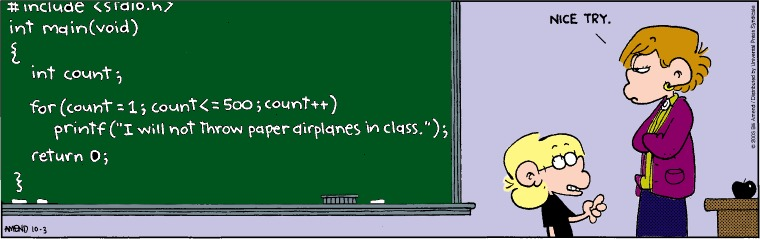
\includegraphics[width=\textwidth]{../figures/cartoon}
        \end{figure}
    \end{example} 
    
%	\LstFor \pause

%    \LstFor
\end{frame}


\begin{frame}
  \frametitle{``For'' Loops}
  \framesubtitle{Typical use}
	\lstinline/for/ loops run while a certain condition is true, but allow separate statement(s) to be run (1)~before the first iteration and (2)~after each iteration.
    The archetypal use for the \lstinline/for/ loop is to loop some pre-determined number of times indexed by a counter variable:
    \LstForBlackboard
    Variable counter is referred to as an ``index''. 
    See \textbf{forloop0.cpp} for a complete program to play with.
\end{frame}


\begin{frame}
  \frametitle{``For'' Loops}
  \framesubtitle{More generally}
	\LstFor
    \begin{itemize}
    \item   Execute Statement1 (only the first time)
    \item   Evaluate Condition
    \begin{itemize}
        \item If Condition is true:
        \begin{itemize} 
            \item Execute the block
            \item Execute Statement2
            \item Back to the Condition
        \end{itemize}
        \item If Condition is false, jump directly at the end of the block
    \end{itemize}
    \end{itemize}
    ``Condition'' may be any boolean expression.
    ``Condition'', ``Statement1'', ``Statement2'' can be empty (but the separators `;' are necessary).
\end{frame}

\begin{frame}
\frametitle{``For'' Loops}
\framesubtitle{Flow chart}
\LstForLine
\begin{figure}
    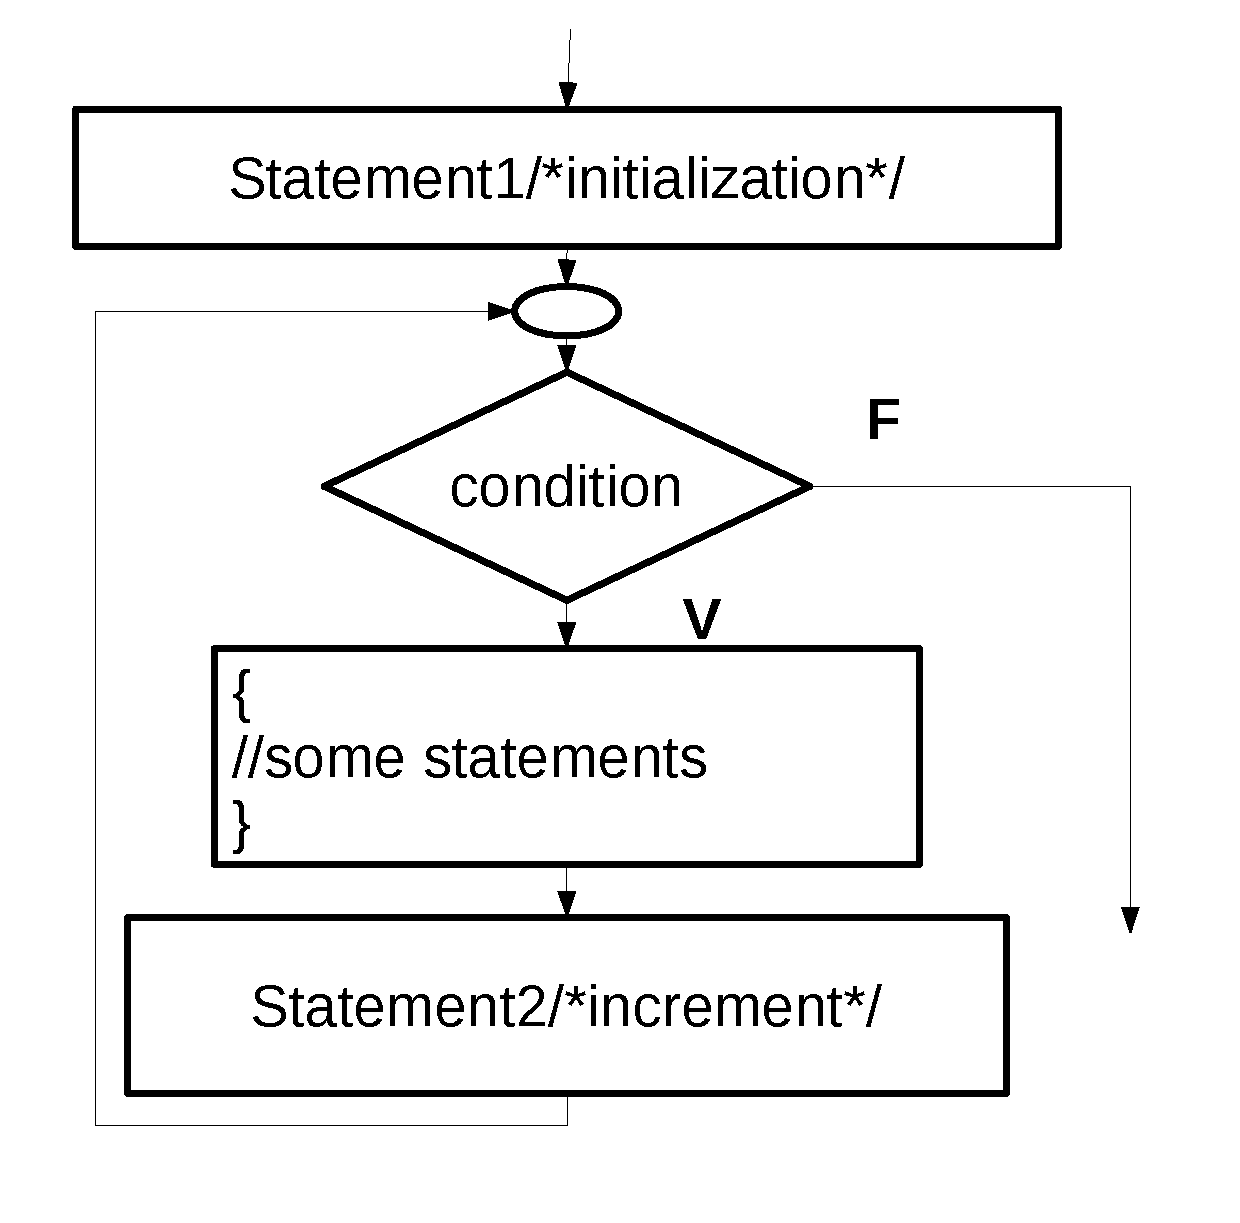
\includegraphics[height=0.7\textheight]{../figures/for_loop}
\end{figure}
\end{frame}


\begin{frame}
  \frametitle{Good programming practices}
  \framesubtitle{though not necessary}
\begin{itemize}
\item  Use \text{indentation}.
\item  Curly brackets $\{\ldots\}$ are necessary only if the code block has more than one statement...
\item  ...but I suggest to use them in any case.
\item  Don't declare more than one variable in Statement1.
\item  Use short name for indexes, e.g., $i$.
\end{itemize}
\end{frame}

\begin{frame}
  \frametitle{Examples}
  Print the first $n$ numbers of the Fibonacci sequence.
\LstFibo
  \begin{alertblock}{Exercise}
    write your own program!
  \end{alertblock}
\end{frame}


\begin{frame}
  \frametitle{Examples}
  Compute and print  $n!$.
\LstFactorial
  \begin{alertblock}{Exercise}
    write your own program!
  \end{alertblock}
\end{frame}

\begin{frame}
  \frametitle{Example}
  \framesubtitle{Numerical solution of a definite integral: theory}
\small
  The \text{trapezium rule} is a method for approximating an integral
  \begin{multline*}
        \int_{a=0}^{b=\pi} sin(x) dx \approx \pi/3 [sin(\pi/3) - sin(0)]/2 \\
            + \pi/3 [sin (2 \pi/3 ) - sin(\pi/3)]/2 + \pi/3 [sin(\pi) - sin(2\pi/3)]/2
  \end{multline*}
  \begin{figure}
    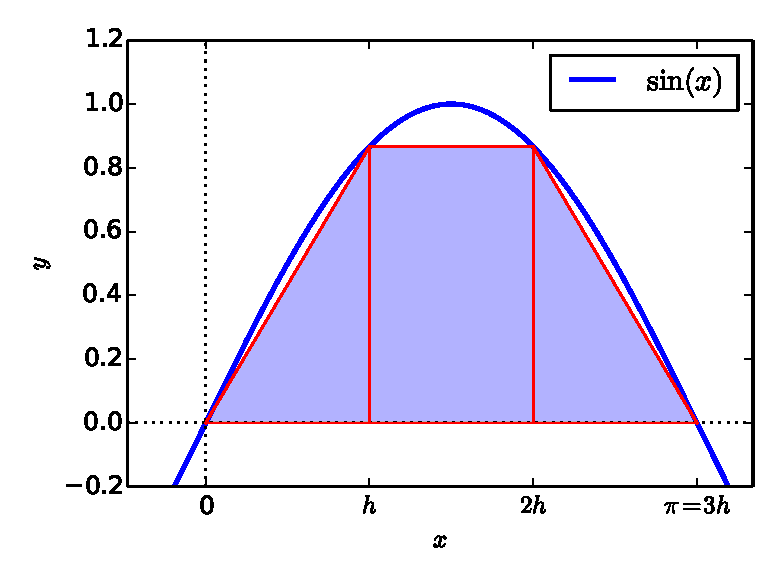
\includegraphics[height=0.7\textheight]{../figures/trapezium}
  \end{figure}
\end{frame}

\begin{frame}
  \frametitle{Example}
  \framesubtitle{Numerical solution of a definite integral: snippet}
\small
For domain discretised into $n$ equally spaced intervals with extremes at points $a,a+h,a+2h,\ldots,b$,
after some algebraic manipulation, the approximation becomes:
  \begin{equation*}
        \int_a^b f(x) dx \approx \frac{h}{2}[f(a)+2\sum_i f(a+ih)+f(b)]
  \end{equation*}
\LstTrapezium
\end{frame}

\begin{frame}
  \frametitle{Example}
  \framesubtitle{Numerical solution of a definite integral: snippet}
\small
Alternative: we can approximate the integral with the sum of rectangles:
  \begin{equation*}
        \int_a^b f(x) dx \approx h\sum_{i=0}^{(b-a)/h} f(a+h*i)
  \end{equation*}
\LstRectangle
Play with \textbf{forloopintegral.cpp}. %Use different functions and/or change the value of $n$.
\end{frame}

\section{``While'' loops}

\begin{frame}
  \frametitle{``While'' loops}
  \framesubtitle{Purely conditioned loops}
	A \lstinline/while/ statement runs a block of code as long as a certain
	condition is true:
	\LstWhile
\end{frame}


\begin{frame}
\frametitle{``While'' Loops}
\framesubtitle{Flow chart}
\LstWhileLine
\begin{figure}
    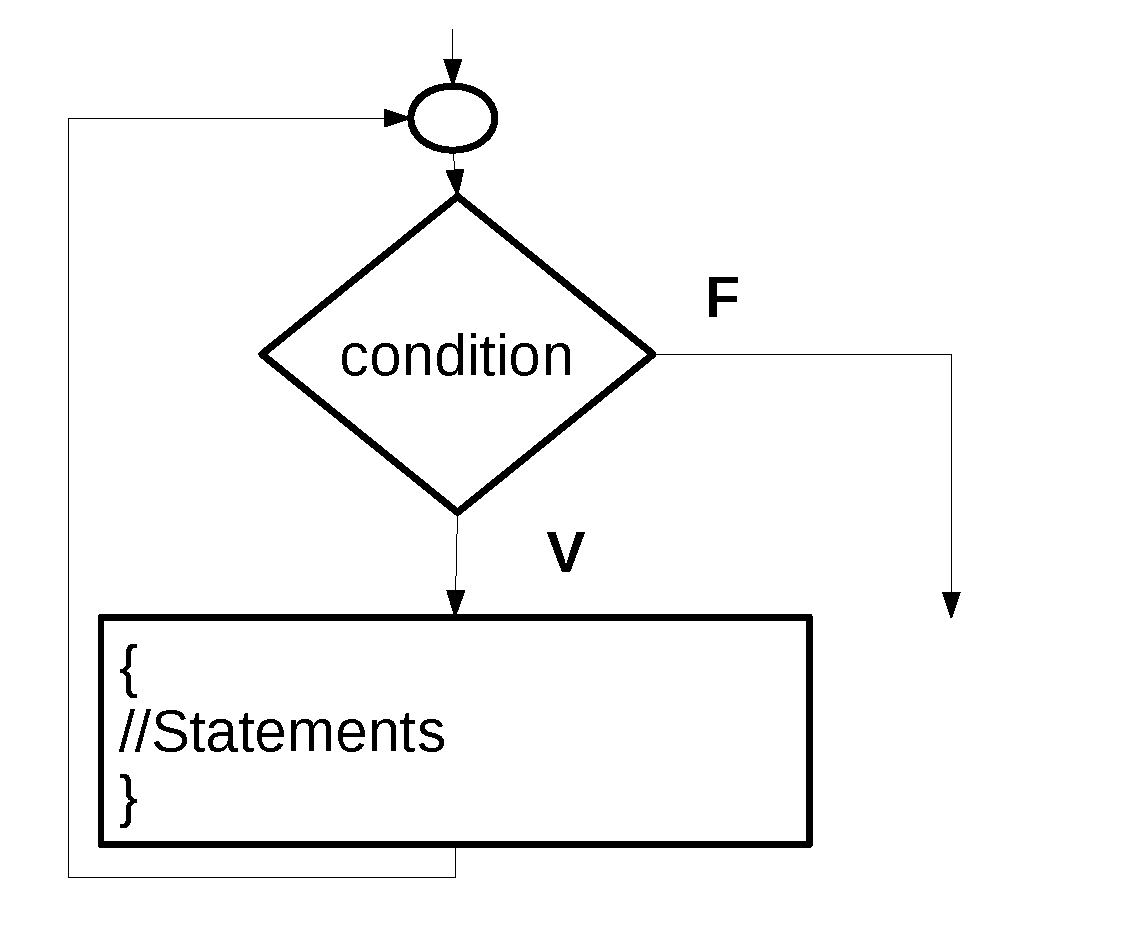
\includegraphics[height=0.7\textheight]{../figures/while_loop}
\end{figure}
\end{frame}

\begin{frame}
  \frametitle{Example}
  \framesubtitle{Series expansion of transcendental function}
\begin{itemize}
    \item You are familiar with $exp(x) = 1+\frac{x}{1!} +\frac{x^2}{2!}+\frac{x^3}{3!} + \ldots$
    \item To approximate $exp(x)$, iterate over the terms of this series, up to a certain order.
    \item You may not know how many terms are needed. Therefore a \lstinline/while/ is preferred over the \lstinline/for/ loop.  
    \item The loop can be interrupted when the term $\frac{x^n}{n!}$ is smaller than a pre-setted threshold.
    \item Play with \textbf{whileloopexponential.cpp} %{whileloop_exponential.cpp}.
\end{itemize}
\begin{alertblock}{Exercise}
 compute $ sin(\pi)$ using its series expansion.
\end{alertblock}
\end{frame}



\begin{frame}
	\frametitle{``Do-while'' loops}
	\framesubtitle{Post-conditioned loops}
	A \lstinline/while/ loop checks its condition even before its first iteration. Sometimes we don't want this: i.e., we want the loop always to run the first time, and only to test the condition before subsequent iterations. To do this, we use the \lstinline/do/--\lstinline/while/ construct:
	\LstDoWhile
\end{frame}


\begin{frame}
\frametitle{``Do-while'' Loops}
\framesubtitle{Flow chart}
\LstDoWhileLine
\begin{figure}
    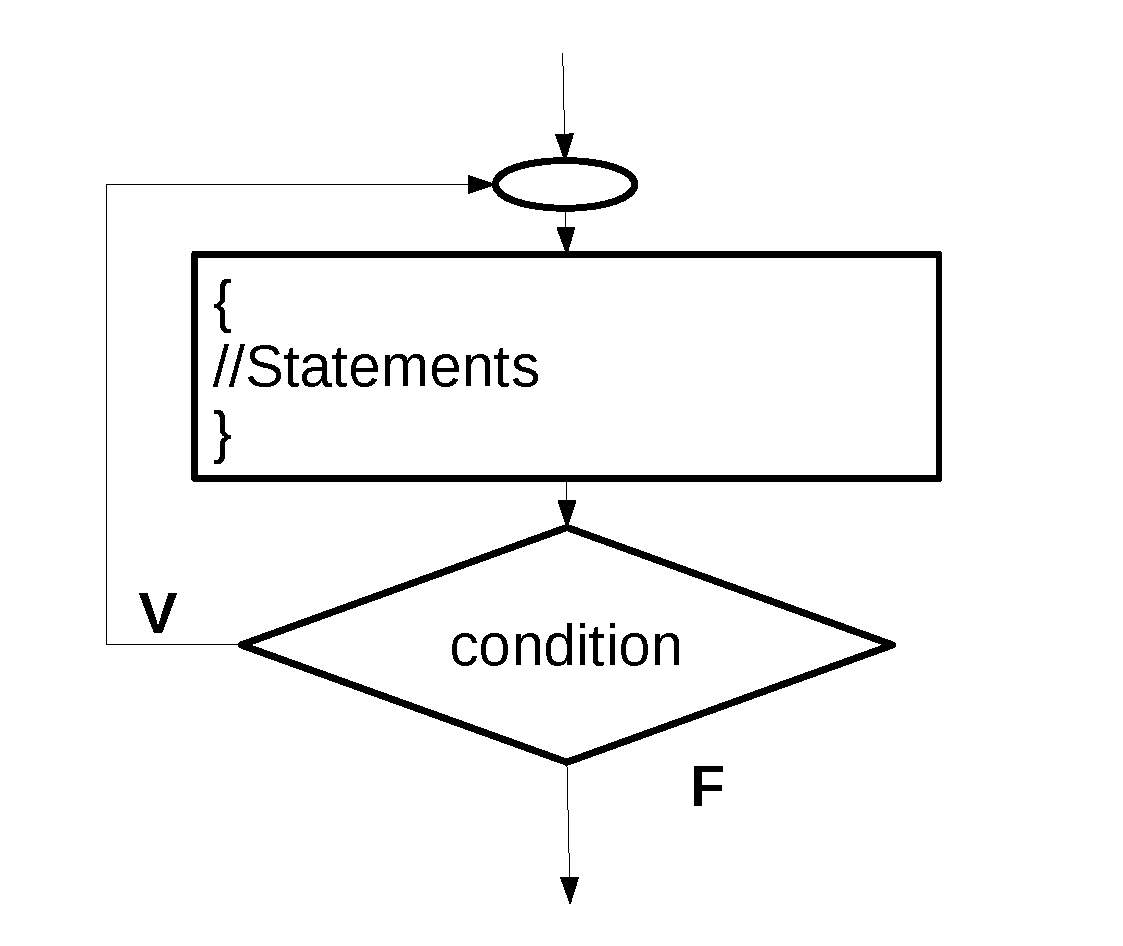
\includegraphics[height=0.7\textheight]{../figures/do_while_loop}
\end{figure}
\end{frame}


\begin{frame}
  \frametitle{Example}
  \framesubtitle{Monte Carlo solution of a definite integral: theory}
\begin{block}{Strategy 1}
Same idea of rectangle rules, but with random uniform sampling of $n$ points in $[a,b]$.

$\int_0^\pi sin(x) \approx \pi/n \sum_{i=1}^{n} \sin(x_i)$,
    where $x_i \in [0,\pi] $
\end{block}
  \begin{figure}
    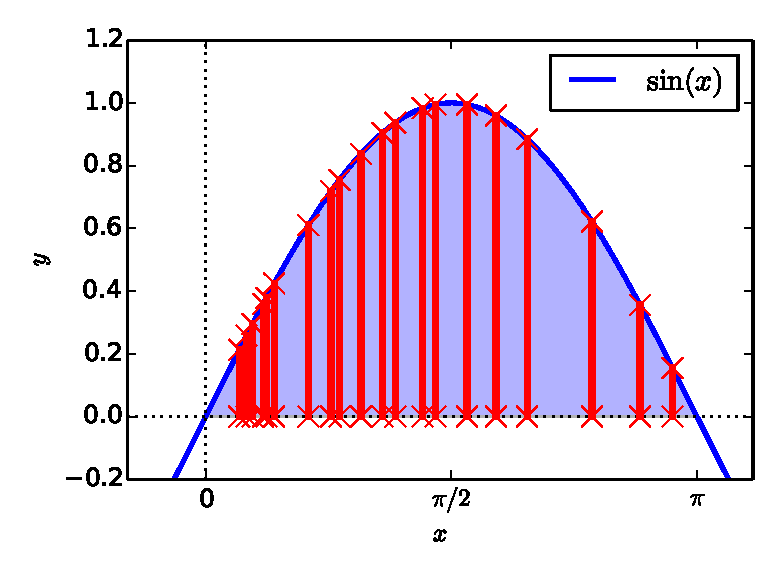
\includegraphics[height=0.7\textheight]{../figures/montecarlo2}
  \end{figure}
\end{frame}

\begin{frame}
  \frametitle{Example}
  \framesubtitle{Monte Carlo solution of a definite  integral: theory}
\begin{block}{Strategy 1}
Same idea of rectangle rules, but with random uniform sampling of $n$ points in $[a,b]$.
$\int_0^\pi sin(x) \approx Q_n \equiv \pi/n \sum_{i=1}^{n} \sin(x_i)$,
    where $x_i \in [0,\pi] $
\end{block}

\begin{itemize}
    \item $i$ is the counter, $n$ is number of iterations.
    \item We don't know a priory the best value for $n$.
    \item Iterate as long as the \textit{relative error} $\pi Var(Q_n)/\sqrt{n}$ is above a certain threshold. 
\end{itemize}

\lstinline/for/ or \lstinline/while/ loop?

\end{frame}




\begin{frame}
  \frametitle{Example}
  \framesubtitle{Monte Carlo solution of a definite  integral: snippet}
    Strategy 1
    \LstDoWhileMontecarloOne
    See \textbf{dowhileloopmontecarlo1.cpp}.
\end{frame}



\begin{frame}
  \frametitle{Example}
  \framesubtitle{Monte Carlo solution of a definite  integral: theory}
\begin{block}{Strategy 2}
Count the points that fall inside the shaded area (you need two random numbers for each sample).
\end{block}
  \begin{figure}
    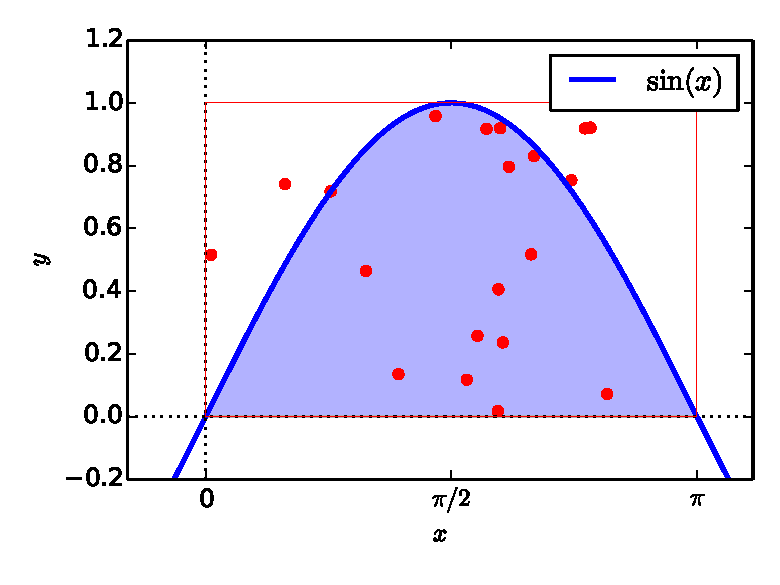
\includegraphics[height=0.7\textheight]{../figures/montecarlo}
  \end{figure}
\end{frame}


\begin{frame}
  \frametitle{Example}
  \framesubtitle{Monte Carlo solution of a definite  integral: snippet}
    Strategy 2
    \LstDoWhileMontecarloTwo
    See \textbf{dowhileloopmontecarlo2.cpp}.
\end{frame}




\begin{frame}
\frametitle{``For'' or ``While''?}
	\begin{itemize}
		\item It depends on you own style, but...
		\item ..when the number of iteration is known a priori, the \lstinline/for/ loop is more clear.
		\item Exercise: implement a Monte-Carlo integration method using the \lstinline/for/ loop.
		\item Exercise: write a program for the Fibonacci series using  a \lstinline/while/ loop.
	\end{itemize}
\end{frame}

\section{Fine flow control}

\begin{frame}
	\frametitle{Break the loop}
	The normal flow of a loop can be modified by using one of the following statements inside the loop's body:
	\begin{itemize}
		\item \lstinline/break/ ends a loop immediately. Control passes
			to the code immediately following the loop.
		\item \lstinline/continue/ ends the current iteration of a
			loop. The loop's condition is then evaluated again, and
			the loop either proceeds to its next iteration, or
			ends, as appropriate.
		\item \lstinline/goto id;/ unconditionally transfer the flow to the statement labeled by \lstinline/id:/.
	\end{itemize}

	Prefer to control loops by their conditions where possible, rather than by using the \lstinline/break/ and \lstinline/continue/ statements. They will be easier to read.
\end{frame}

\begin{frame}
	\frametitle{Nested Loops}
	\begin{itemize}
        \item  Any loop can be completely nested inside another loop.
		\item In case of two nested \lstinline/for/ loops, each loop should have a different \textit{index}.
		\item \lstinline/continue/ and \lstinline/break/ work only on a single ``level''.
		\item In order to exit from all the nested loops you could use \lstinline/goto/ ...
		\item ... or play with the condition, as in  structured programming convention.
	\end{itemize}
\end{frame}


\begin{frame}
	\frametitle{Exit from a nested Loops}
    \framesubtitle{Example 1: non-structured code}
\LstNestedGoto
    See \textbf{forloopnested.cpp}.
\end{frame}



\begin{frame}
	\frametitle{Exit from a nested Loops}
    \framesubtitle{Example 2: structured code}
\LstNestedStructured
    See \textbf{forloopnested.cpp}.
\end{frame}

\section{Exercises}

\begin{frame}
	\frametitle{Exercises}

	\begin{itemize}
        \item Find the area of unitary disk using Monte-Carlo strategy 2. 
		\item Prompt the user for an angle and then display a message
			indicating whether its sine is positive, negative or
			zero.
		\item Play guess-the-number with the user: the computer chooses
			a number, and the user keeps guessing it until they get it right.
			The computer should report whether each guess is too
			large or too small.
	\end{itemize}
\end{frame}



\end{document}
